\section{Durchführung}
\label{sec:Durchfuehrung}
Für den gesamten Versuch wird ein Lock-In-Verstärker mit eingbautem Vorverstärker, Tief- und Bandpass, Phasenverschieber,
sowie Funktions- und Rauschgenerator verwendet. Außerdem wird ein Oszilloskop verwendet, um die verschiedenen Signale darzustellen.

\begin{figure} [H]
    \centering
    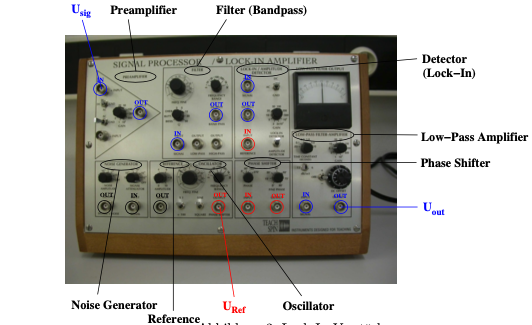
\includegraphics[height=8cm]{content/Bilder/Aufbau_Bild.png}
    \caption{Lock-In-Verstärker ohne Verkabelung.\cite{v303}}
    \label{fig:Aufbau Lock-In-Verstaerker}
\end{figure}

% Ohne Rauschen
\subsection{Messung ohne Rauschen}
\label{sec:Messung ohne Rauschen}
Das in \autoref{fig:Aufbau Lock-In-Verstaerker} zu sehende Gerät wird wie in \autoref{fig:Schematischer Aufbau} verkabelt, 
wobei in einer ersten Messreihe der Rauschgenerator überbrückt wird. Der Funktionsgenerator wird auf eine Sinusspannung mit 
$U_{\symup{sig}}\approx\qty{2}{\volt}$ und eine Frequenz von rund $\qty{1}{\kilo\hertz}$ eingestellt. Dieses Signal wird 
verstärkt und durch den Bandpassfilter geleitet. Das Referenzsignal $U_{\symup{ref}}$ wird ebenfalls im Funktionsgenerator 
erzeugt und hat dieselbe Frequenz wie $U_{\symup{sig}}$, wird allerdings im Phasenverschieber um $\symup{\Delta}\varphi$ 
phasenverschoben. Dieses Signal $U_{\symup{ref}}$ wird im Detektor mit dem Signal $U_{\symup{sig}}$ multipliziert und in einem
Tiefpass nochmals gefiltert. Das Ausgangssignal $U_{\symup{out}}$ wird auf einem Oszilloskop angezeigt.

Im Verlauf der Messung wird die Verschiebung der Phase zwischen $U_{\symup{sig}}$ und $U_{\symup{ref}}$ mit dem Phasenverschieber
in 30° Schritten verändert und es wird mithilfe des Oszilloskop die Spannung des Ausgangssignal $U_{\symup{out}}$ gemessen und tabellarisch
protokolliert.

\begin{figure} [H]
    \centering
    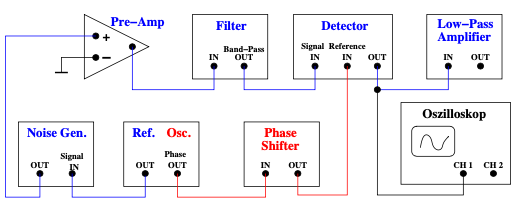
\includegraphics[height=5cm]{content/Bilder/Aufbau_Schema.png}
    \caption{Schematischer Aufbau des Lock-In-Verstärkers.\cite{v303}}
    \label{fig:Schematischer Aufbau}
\end{figure}

\subsection{Messung mit Rauschen}
\label{sec:Messung mit Rauschen}
Die Messung aus \ref{sec:Messung ohne Rauschen} wird nun mit einem eingeschalteten Rauschgenerator wiederholt. Die Amplitude
des Rauschens liegt hierbei in derselben Größenordnung wie die des Signals~$U_{\symup{sig}}$.


\subsection{Messung mit einer LED}
\label{sec:Messung mit einer LED}
Es wird eine Photodetektorschaltung gemäß \autoref{fig:Photodetektorschaltung} aufgebaut. Der Unterschied zu der vorherigen 
Schaltung (\autoref{fig:Schematischer Aufbau}) liegt darin, dass nun nicht mehr ein Rauschgenerator verwendet wird. Stattdessen
wird das Ausgabesignal eines Photodetektors, welcher Lichtwellen einer blinkenden LED registriert, analysiert.
Aufgrund des Umgebungslichtes nimmt der Photodetektor von sich aus bereits ein Hintergrundrauschen auf, welches
anschließend mit dem Lock-In Verstärker rausgefiltert werden soll.

\begin{figure} [H]
    \centering
    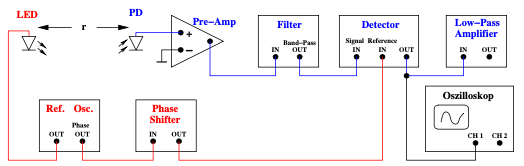
\includegraphics[height=5cm]{content/Bilder/Aufbau_led.png}
    \caption{Schematischer Aufbau der Photodetektorschaltung.\cite{v303}}
    \label{fig:Photodetektorschaltung}
\end{figure}

Die blinkende LED wird schrittweise von dem Photodetektor entfernt und es wird die Signalstärke $U_{\symup{out}}$ abhängig von dem 
Abstand $r$ zwischen LED und Photodetektor mithilfe des Oszilloskops bestimmt.